\documentclass[12pt]{article}\usepackage[]{graphicx}\usepackage[]{xcolor}
% maxwidth is the original width if it is less than linewidth
% otherwise use linewidth (to make sure the graphics do not exceed the margin)
\makeatletter
\def\maxwidth{ %
  \ifdim\Gin@nat@width>\linewidth
    \linewidth
  \else
    \Gin@nat@width
  \fi
}
\makeatother

\definecolor{fgcolor}{rgb}{0, 0, 0}
\newcommand{\hlnum}[1]{\textcolor[rgb]{0.69,0.494,0}{#1}}%
\newcommand{\hlsng}[1]{\textcolor[rgb]{0.749,0.012,0.012}{#1}}%
\newcommand{\hlcom}[1]{\textcolor[rgb]{0.514,0.506,0.514}{\textit{#1}}}%
\newcommand{\hlopt}[1]{\textcolor[rgb]{0,0,0}{#1}}%
\newcommand{\hldef}[1]{\textcolor[rgb]{0,0,0}{#1}}%
\newcommand{\hlkwa}[1]{\textcolor[rgb]{0,0,0}{\textbf{#1}}}%
\newcommand{\hlkwb}[1]{\textcolor[rgb]{0,0.341,0.682}{#1}}%
\newcommand{\hlkwc}[1]{\textcolor[rgb]{0,0,0}{\textbf{#1}}}%
\newcommand{\hlkwd}[1]{\textcolor[rgb]{0.004,0.004,0.506}{#1}}%
\let\hlipl\hlkwb

\usepackage{framed}
\makeatletter
\newenvironment{kframe}{%
 \def\at@end@of@kframe{}%
 \ifinner\ifhmode%
  \def\at@end@of@kframe{\end{minipage}}%
  \begin{minipage}{\columnwidth}%
 \fi\fi%
 \def\FrameCommand##1{\hskip\@totalleftmargin \hskip-\fboxsep
 \colorbox{shadecolor}{##1}\hskip-\fboxsep
     % There is no \\@totalrightmargin, so:
     \hskip-\linewidth \hskip-\@totalleftmargin \hskip\columnwidth}%
 \MakeFramed {\advance\hsize-\width
   \@totalleftmargin\z@ \linewidth\hsize
   \@setminipage}}%
 {\par\unskip\endMakeFramed%
 \at@end@of@kframe}
\makeatother

\definecolor{shadecolor}{rgb}{.97, .97, .97}
\definecolor{messagecolor}{rgb}{0, 0, 0}
\definecolor{warningcolor}{rgb}{1, 0, 1}
\definecolor{errorcolor}{rgb}{1, 0, 0}
\newenvironment{knitrout}{}{} % an empty environment to be redefined in TeX

\usepackage{alltt}

\usepackage[hmargin=1in,vmargin=1in]{geometry}
\usepackage{parskip}
\usepackage{hyperref}
\usepackage{graphicx}
\usepackage{color}
\usepackage{verbatim}
\hypersetup{pdfstartview=FitV,hidelinks}


\definecolor{inlinecolor}{rgb}{0.878,0.918,0.933}  
\newcommand{\inr}[1]{\colorbox{inlinecolor}{\texttt{#1}}}







\IfFileExists{upquote.sty}{\usepackage{upquote}}{}
\begin{document}

{
  \Large
  \centering
  {\bf Lab -- Estimating survival, recruitment, and growth rate
    with capture-mark-recapture data} \\
  Due by noon on Monday \\
}

\vspace{10pt}

The purpose of this lab is to learn how to use the R package `marked' to
estimate survival, recruitment, and growth rate using mark-recapture
data. Put your code and answers in a Word file named something like
``Chandler-lab.docx'', and upload it to ELC. The use of RMarkdown is
encouraged but not required.  

%\vspace{-12pt}


\section*{\large Exercise I: Estimating Canada Warbler survival with the CJS model}

%\vspace{-10pt}

%{\bf Background}

The Canada Warbler ({\it Cardellina canadensis}) is a long-distance
migratory bird that primarily breeds in the boreal forests of
Canada. However, a small portion of the range extends down through the
Appalachian Mountains to northern Georgia.

Canada Warblers are too small to use telemetry to estimate annual
survival, so we use mark-recapture methods instead. Each year, we
visit multiple sites and run mist-nets for 4 consecutive days at each
site. All newly captured individuals are marked with a uniquely
numbered metal band, and a unique combination of color bands.

The data come from five years (2014--2018) of surveys. Even though
``the robust design'' was used, the data were collapsed so that only
one value (0 or 1) is shown for each year for each individual.
%% Program MARK will ignore all leading zeros in the encounter histories.

{\bf Assignment}

\begin{enumerate}
  \item Import the capture histories in the file
    \texttt{cawa-cjs.inp}.
  \item Fit 4 models:
    \begin{itemize}
      \item $\Phi(.)p(.)$ -- No variation in apparent survival or capture probability
      \item $\Phi(t)p(.)$ -- Temporal variation in apparent survival
      \item $\Phi(.)p(t)$ -- Temporal variation in capture probability
      \item $\Phi(t)p(t)$ -- Temporal variation in apparent survival and capture probability
    \end{itemize}
  \item What is the best model according to AIC?
  \item Create a table to report the estimates (on the probability
    scale), standard errors, and 95\% confidence intervals for $p$ and
    $\Phi$ from the best model. 
\end{enumerate}

  
\clearpage

\section*{\large  Exercise II: The Jolly-Seber model
  for estimating survival, recruitment, and growth rate}

% \textcolor{red}{THE CH DATA HAVE CHANGED AND THERE ARE MORE THAN 5 SIX
%   YEARS NOW. NEED TO FIX THIS}

%{\bf Background}

Stinkpots ({\it Sternotherus odoratus}) were captured, marked,
released, and occasionally recaptured at Dean's Pond at Whitehall
Forest using baited hoop traps. Sampling began in 2007. 


% {\bf Instructions}

% \begin{enumerate}
%   \item Set verb Encounter Occasions  to 6 (for 6 years of data)
%   \item Sampling occurred on years 2007, 2010, 2011, 2012, 2014, and
%     2015, so the time intervals between sampling occasions differs. To
%     account for this, select verb "Set Time Intervals" and specify the
%     time gaps as 3, 1, 1, 2, 1. Hit verb "OK", then hit it again on
%     the next screen.
% \end{enumerate}





% \begin{figure}[h!]
%   \centering
%   \fbox{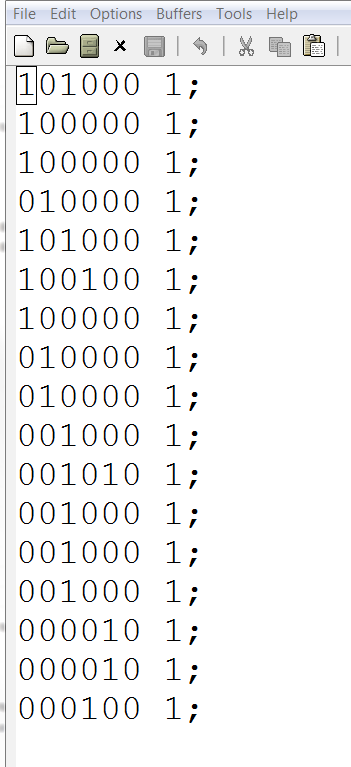
\includegraphics[height=7.5cm]{figs/stinkpot07-data}}
%   \caption{\small Stinkpot capture histories in a text file ready to
%     be imported to MARK.}
%   \label{fig:stink07-data}
% \end{figure}

{\bf Assignment}

\begin{enumerate}
  \item Import data from the file \texttt{CH-SO-Dean-AllYears.inp}.
  \item Fit a Jolly-Seber model with constant capture probability
    ($p$), constant entrance probabilities (\texttt{pent}, $b_t$), and
    temporal variation in apparent survival.
%  \item Interpret the parameter estimates. (For parameters that are
%    year-specific, you do not need to interpret each yearly-estimate.) 
  \item Use the parameter estimates to compute:
    \begin{itemize}
      \item Super-population size
      \item The number of recruits in each time interval
      \item Abundance at each time point. Hint: apparent survival
        ($\Phi$) varies over time.
      \item Growth rate for each time interval ($\lambda_t$)
    \end{itemize}
  \item Plot $\lambda_t$ over time.
  % \item What conclusions can you draw from this analysis? Do you think
  %   the population is growing, shrinking, remaining constant, or is it
  %   difficult to tell? 
\end{enumerate}


\clearpage

\section*{Example analysis}




We will fit models using the R package `marked'. You can install it
using the following command, which only needs to be run once: 

\begin{knitrout}
\definecolor{shadecolor}{rgb}{0.878, 0.918, 0.933}\color{fgcolor}\begin{kframe}
\begin{alltt}
\hlkwd{install.packages}\hldef{(}\hlsng{"marked"}\hldef{)}
\end{alltt}
\end{kframe}
\end{knitrout}


You can load the package with this command:

\begin{knitrout}
\definecolor{shadecolor}{rgb}{0.878, 0.918, 0.933}\color{fgcolor}\begin{kframe}
\begin{alltt}
\hlkwd{library}\hldef{(marked)}
\end{alltt}
\end{kframe}
\end{knitrout}

Capture history data are in a text file formatted for program MARK. We
can important the data and prepare them for `marked' using code like
this: 

\begin{knitrout}
\definecolor{shadecolor}{rgb}{0.878, 0.918, 0.933}\color{fgcolor}\begin{kframe}
\begin{alltt}
\hldef{example.cjs.data} \hlkwb{<-} \hlkwd{read.table}\hldef{(}\hlsng{"example-cjs.inp"}\hldef{,} \hlkwc{sep}\hldef{=}\hlsng{" "}\hldef{,}
                               \hlkwc{colClasses}\hldef{=}\hlkwd{c}\hldef{(}\hlsng{"character"}\hldef{,}\hlsng{"character"}\hldef{),}
                               \hlkwc{col.names}\hldef{=}\hlkwd{c}\hldef{(}\hlsng{"ch"}\hldef{,} \hlsng{"count"}\hldef{))}
\end{alltt}
\end{kframe}
\end{knitrout}

The data must have a column called \inr{ch}, formatted as a character
vector. The second column (\inr{count}) is not important, and it
can be ignored.

\begin{knitrout}
\definecolor{shadecolor}{rgb}{0.878, 0.918, 0.933}\color{fgcolor}\begin{kframe}
\begin{alltt}
\hlkwd{head}\hldef{(example.cjs.data,} \hlkwc{n}\hldef{=}\hlnum{4}\hldef{)} \hlcom{# Show the first 4 lines of data}
\end{alltt}
\begin{verbatim}
##      ch count
## 1 10000    1;
## 2 00100    1;
## 3 01000    1;
## 4 01000    1;
\end{verbatim}
\end{kframe}
\end{knitrout}

Everything looks good, so we're ready to fit a model with the
\inr{crm} function. 

\subsection*{Cormack-Jolly-Seber model}

The CJS model parameters are: apparent survival (Phi, $\Phi$) and capture
probability ($p$). Let's start with the simplest CJS model in which
$\Phi$ and $p$ are constant: 


\begin{knitrout}
\definecolor{shadecolor}{rgb}{0.878, 0.918, 0.933}\color{fgcolor}\begin{kframe}
\begin{alltt}
\hldef{phi0.p0} \hlkwb{<-} \hlkwd{crm}\hldef{(}\hlkwc{data}\hldef{=example.cjs.data,} \hlkwc{model}\hldef{=}\hlsng{"CJS"}\hldef{,} \hlkwc{hessian}\hldef{=}\hlnum{TRUE}\hldef{,}
               \hlkwc{model.parameters}\hldef{=}\hlkwd{list}\hldef{(}
                   \hlkwc{Phi}\hldef{=}\hlkwd{list}\hldef{(}\hlkwc{formula}\hldef{=}\hlopt{~}\hlnum{1}\hldef{),}  \hlcom{## No variation}
                   \hlkwc{p}\hldef{=}\hlkwd{list}\hldef{(}\hlkwc{formula}\hldef{=}\hlopt{~}\hlnum{1}\hldef{)))}   \hlcom{## No variation}
\end{alltt}
\end{kframe}
\end{knitrout}

The \inr{data} argument is for the capture history data. The
\inr{model} specifies the type of model you want to fit. We will use
\texttt{CJS} and \texttt{JS}. If \inr{hessian=FALSE}, you won't get
standard errors or confidence intervals. The \inr{model.parameters}
argument is one to focus on. This is where you specify the sources of
variation in apparent survival and capture probability. 


\clearpage

Typing the name of the object dispays the AIC score and
the estimates on the logit scale.  

\begin{knitrout}\small
\definecolor{shadecolor}{rgb}{0.878, 0.918, 0.933}\color{fgcolor}\begin{kframe}
\begin{alltt}
\hldef{phi0.p0}
\end{alltt}
\begin{verbatim}
## 
## crm Model Summary
## 
## Npar :  2
## -2lnL:  154.104
## AIC  :  158.104
## 
## Beta
##                  Estimate        se       lcl       ucl
## Phi.(Intercept)  2.321548 2.2567894 -2.101759  6.744855
## p.(Intercept)   -1.977161 0.4428573 -2.845161 -1.109161
\end{verbatim}
\end{kframe}
\end{knitrout}

To see the esimates on the probability scale, we need to use the
\inr{predict} function.

\begin{knitrout}
\definecolor{shadecolor}{rgb}{0.878, 0.918, 0.933}\color{fgcolor}\begin{kframe}
\begin{alltt}
\hlkwd{predict}\hldef{(phi0.p0)}
\end{alltt}
\begin{verbatim}
## $Phi
##   occ estimate        se       lcl       ucl
## 1   4 0.910646 0.1836347 0.1089259 0.9988245
## 
## $p
##   occ  estimate         se        lcl       ucl
## 1   5 0.1216218 0.04731041 0.05493197 0.2480274
\end{verbatim}
\end{kframe}
\end{knitrout}


If we think survival probability varies over time, but detection
probability is constant, we can change the \texttt{formula}:


\begin{knitrout}
\definecolor{shadecolor}{rgb}{0.878, 0.918, 0.933}\color{fgcolor}\begin{kframe}
\begin{alltt}
\hldef{phiTime.p0} \hlkwb{<-} \hlkwd{crm}\hldef{(}\hlkwc{data}\hldef{=example.cjs.data,} \hlkwc{model}\hldef{=}\hlsng{"cjs"}\hldef{,} \hlkwc{hessian}\hldef{=}\hlnum{TRUE}\hldef{,}
                  \hlkwc{model.parameters}\hldef{=}\hlkwd{list}\hldef{(}
                      \hlkwc{Phi}\hldef{=}\hlkwd{list}\hldef{(}\hlkwc{formula}\hldef{=}\hlopt{~}\hldef{time),}  \hlcom{## Temporal variation}
                      \hlkwc{p}\hldef{=}\hlkwd{list}\hldef{(}\hlkwc{formula}\hldef{=}\hlopt{~}\hlnum{1}\hldef{)))}      \hlcom{## No variation}
\end{alltt}
\end{kframe}
\end{knitrout}

Notice how the results now show survival probability for each time period:

\begin{knitrout}
\definecolor{shadecolor}{rgb}{0.878, 0.918, 0.933}\color{fgcolor}\begin{kframe}
\begin{alltt}
\hlkwd{predict}\hldef{(phiTime.p0)}
\end{alltt}
\begin{verbatim}
## $Phi
##   time occ  estimate          se          lcl       ucl
## 1    4   4 0.6527671 0.264050300 1.608282e-01 0.9485600
## 2    3   3 0.6808526 0.250026508 1.827878e-01 0.9531561
## 3    2   2 0.9998875 0.006369269 5.588049e-45 1.0000000
## 4    1   1 0.8994609 0.401574681 1.482594e-03 0.9999814
## 
## $p
##   occ  estimate         se        lcl       ucl
## 1   5 0.1557208 0.04990822 0.08058259 0.2796134
\end{verbatim}
\end{kframe}
\end{knitrout}


\clearpage

\subsection*{Jolly-Seber model}

The JS model can be used to estimate abundance, apparent survival,
recruitment, growth rate, and capture probability. First, let's import
the example data: 

\begin{knitrout}
\definecolor{shadecolor}{rgb}{0.878, 0.918, 0.933}\color{fgcolor}\begin{kframe}
\begin{alltt}
\hldef{example.js.data} \hlkwb{<-} \hlkwd{read.table}\hldef{(}\hlsng{"example-js.inp"}\hldef{,} \hlkwc{sep}\hldef{=}\hlsng{" "}\hldef{,}
                              \hlkwc{colClasses}\hldef{=}\hlkwd{c}\hldef{(}\hlsng{"character"}\hldef{,}\hlsng{"character"}\hldef{),}
                              \hlkwc{col.names}\hldef{=}\hlkwd{c}\hldef{(}\hlsng{"ch"}\hldef{,} \hlsng{"count"}\hldef{))}
\end{alltt}
\end{kframe}
\end{knitrout}

The new parameter that will be estimated is called \texttt{pent} ($b_i$),
which is the ``entrance probability'' describing the probability that
an individual entered the population during a particular
occasion. Here's a model in which all 3 parameters are constant.


\begin{knitrout}
\definecolor{shadecolor}{rgb}{0.878, 0.918, 0.933}\color{fgcolor}\begin{kframe}
\begin{alltt}
\hldef{js.phi0.pent0.p0} \hlkwb{<-} \hlkwd{crm}\hldef{(}\hlkwc{data}\hldef{=example.js.data,} \hlkwc{model}\hldef{=}\hlsng{"JS"}\hldef{,} \hlkwc{hessian}\hldef{=}\hlnum{TRUE}\hldef{,}
                        \hlkwc{model.parameters}\hldef{=}\hlkwd{list}\hldef{(}
                            \hlkwc{Phi}\hldef{=}\hlkwd{list}\hldef{(}\hlkwc{formula}\hldef{=}\hlopt{~}\hlnum{1}\hldef{),}   \hlcom{## No variation}
                            \hlkwc{pent}\hldef{=}\hlkwd{list}\hldef{(}\hlkwc{formula}\hldef{=}\hlopt{~}\hlnum{1}\hldef{),}  \hlcom{## No variation}
                            \hlkwc{p}\hldef{=}\hlkwd{list}\hldef{(}\hlkwc{formula}\hldef{=}\hlopt{~}\hlnum{1}\hldef{)))}    \hlcom{## No variation}
\end{alltt}
\end{kframe}
\end{knitrout}


Here are the estimates on the probability scale:


\begin{knitrout}\small
\definecolor{shadecolor}{rgb}{0.878, 0.918, 0.933}\color{fgcolor}\begin{kframe}
\begin{alltt}
\hldef{js0est} \hlkwb{<-} \hlkwd{predict}\hldef{(js.phi0.pent0.p0)}
\hldef{js0est}
\end{alltt}
\begin{verbatim}
## $Phi
##   occ  estimate         se       lcl      ucl
## 1   1 0.7239384 0.03646061 0.6471427 0.789458
## 
## $p
##   occ  estimate         se       lcl      ucl
## 1   1 0.5941143 0.06060417 0.4721316 0.705492
## 
## $pent
##   time occ   estimate         se        lcl        ucl
## 1    2   2 0.05722326 0.01154076 0.03837741 0.08451043
## 2    3   3 0.05722326 0.01154076 0.03837741 0.08451043
## 3    4   4 0.05722326 0.01154076 0.03837741 0.08451043
## 4    5   5 0.05722326 0.01154076 0.03837741 0.08451043
## 5    6   6 0.05722326 0.01154076 0.03837741 0.08451043
## 6    7   7 0.05722326 0.01154076 0.03837741 0.08451043
## 7    8   8 0.05722326 0.01154076 0.03837741 0.08451043
## 8    9   9 0.05722326 0.01154076 0.03837741 0.08451043
## 
## $N
##   estimate       se      lcl     ucl
## 1  14.0758 5.313293 6.716731 29.4977
\end{verbatim}
\end{kframe}
\end{knitrout}

The interpretations of Phi ($\Phi$) and $p$ are the same as in the CJS
model. The estimate of $N$ is not what you might expect. Instead of
$N$ being the number of individuals alive at a single point in time,
it is the number of individuals alive during the entire sampling
period that were not detected. For this reason,
$N^{\mathrm{super}}=n+N$ is often called the ``super-population size''.

So, how do we calculate $N_t$, abundance at each time point? We will
tackle this in several steps. First, let's compute the number of
recruits during each time period ($R_t=N^{\mathrm{super}}\times b_t$).  

\begin{knitrout}\small
\definecolor{shadecolor}{rgb}{0.878, 0.918, 0.933}\color{fgcolor}\begin{kframe}
\begin{alltt}
\hldef{n} \hlkwb{<-} \hlkwd{nrow}\hldef{(example.js.data)}     \hlcom{# number of individuals captured}
\hldef{Nsuper} \hlkwb{<-} \hldef{n}\hlopt{+}\hldef{js0est}\hlopt{$}\hldef{N}\hlopt{$}\hldef{estimate}  \hlcom{# Super-population size}
\hldef{Nsuper}
\end{alltt}
\begin{verbatim}
## [1] 81.0758
\end{verbatim}
\begin{alltt}
\hldef{b} \hlkwb{<-} \hldef{js0est}\hlopt{$}\hldef{pent}\hlopt{$}\hldef{estimate}      \hlcom{# Entrance probabilities after first time period}
\hldef{b0} \hlkwb{<-} \hlnum{1}\hlopt{-}\hlkwd{sum}\hldef{(b)}                 \hlcom{# Compute first entrance probability}
\hlkwd{round}\hldef{(b,} \hlkwc{digits}\hldef{=}\hlnum{3}\hldef{)}
\end{alltt}
\begin{verbatim}
## [1] 0.057 0.057 0.057 0.057 0.057 0.057 0.057 0.057
\end{verbatim}
\begin{alltt}
\hldef{R} \hlkwb{<-} \hldef{Nsuper}\hlopt{*}\hldef{b}                  \hlcom{# Recruits}
\hldef{R}
\end{alltt}
\begin{verbatim}
## [1] 4.639422 4.639422 4.639422 4.639422 4.639422 4.639422 4.639422 4.639422
\end{verbatim}
\end{kframe}
\end{knitrout}

Next, extract the estimate of apparent survival, which doesn't vary
over time in this example:

\begin{knitrout}
\definecolor{shadecolor}{rgb}{0.878, 0.918, 0.933}\color{fgcolor}\begin{kframe}
\begin{alltt}
\hldef{Phi} \hlkwb{<-} \hldef{js0est}\hlopt{$}\hldef{Phi}\hlopt{$}\hldef{estimate}   \hlcom{## Apparent survival probability}
\hldef{Phi}
\end{alltt}
\begin{verbatim}
## [1] 0.7239384
\end{verbatim}
\end{kframe}
\end{knitrout}

Now we're ready to calculate abundance

\begin{knitrout}
\definecolor{shadecolor}{rgb}{0.878, 0.918, 0.933}\color{fgcolor}\begin{kframe}
\begin{alltt}
\hldef{nYears} \hlkwb{<-} \hlkwd{length}\hldef{(R)}\hlopt{+}\hlnum{1}
\hldef{N} \hlkwb{<-} \hlkwd{rep}\hldef{(}\hlnum{NA}\hldef{, nYears)}
\hldef{N[}\hlnum{1}\hldef{]} \hlkwb{<-} \hldef{Nsuper}\hlopt{*}\hldef{b0}            \hlcom{## Initial abundance}
\hldef{N[}\hlnum{2}\hldef{]} \hlkwb{<-} \hldef{N[}\hlnum{1}\hldef{]}\hlopt{*}\hldef{Phi} \hlopt{+} \hldef{R[}\hlnum{1}\hldef{]}      \hlcom{## Abundance in year 2}
\hldef{N[}\hlnum{3}\hldef{]} \hlkwb{<-} \hldef{N[}\hlnum{2}\hldef{]}\hlopt{*}\hldef{Phi} \hlopt{+} \hldef{R[}\hlnum{2}\hldef{]}      \hlcom{## Abundance in year 3}
\hldef{N[}\hlnum{4}\hldef{]} \hlkwb{<-} \hldef{N[}\hlnum{3}\hldef{]}\hlopt{*}\hldef{Phi} \hlopt{+} \hldef{R[}\hlnum{3}\hldef{]}      \hlcom{## Abundance in year 4}
\hldef{N[}\hlnum{5}\hldef{]} \hlkwb{<-} \hldef{N[}\hlnum{4}\hldef{]}\hlopt{*}\hldef{Phi} \hlopt{+} \hldef{R[}\hlnum{4}\hldef{]}      \hlcom{## Abundance in year 5}
\hldef{N[}\hlnum{6}\hldef{]} \hlkwb{<-} \hldef{N[}\hlnum{5}\hldef{]}\hlopt{*}\hldef{Phi} \hlopt{+} \hldef{R[}\hlnum{5}\hldef{]}      \hlcom{## Abundance in year 6}
\hldef{N[}\hlnum{7}\hldef{]} \hlkwb{<-} \hldef{N[}\hlnum{6}\hldef{]}\hlopt{*}\hldef{Phi} \hlopt{+} \hldef{R[}\hlnum{6}\hldef{]}      \hlcom{## Abundance in year 7}
\hldef{N[}\hlnum{8}\hldef{]} \hlkwb{<-} \hldef{N[}\hlnum{7}\hldef{]}\hlopt{*}\hldef{Phi} \hlopt{+} \hldef{R[}\hlnum{7}\hldef{]}      \hlcom{## Abundance in year 8}
\hldef{N[}\hlnum{9}\hldef{]} \hlkwb{<-} \hldef{N[}\hlnum{8}\hldef{]}\hlopt{*}\hldef{Phi} \hlopt{+} \hldef{R[}\hlnum{8}\hldef{]}      \hlcom{## Abundance in year 9}
\hlkwd{round}\hldef{(N,} \hlkwc{digits}\hldef{=}\hlnum{0}\hldef{)}
\end{alltt}
\begin{verbatim}
## [1] 44 36 31 27 24 22 21 20 19
\end{verbatim}
\end{kframe}
\end{knitrout}

\clearpage

An alternative to typing out the equation each year, we could compute
abundance in years 2 through 9 in a ``for loop'':

\begin{knitrout}
\definecolor{shadecolor}{rgb}{0.878, 0.918, 0.933}\color{fgcolor}\begin{kframe}
\begin{alltt}
\hldef{N[}\hlnum{1}\hldef{]} \hlkwb{<-} \hldef{Nsuper}\hlopt{*}\hldef{b0}
\hlkwa{for}\hldef{(t} \hlkwa{in} \hlnum{2}\hlopt{:}\hldef{nYears) \{}
    \hldef{N[t]} \hlkwb{<-} \hldef{N[t}\hlopt{-}\hlnum{1}\hldef{]}\hlopt{*}\hldef{Phi} \hlopt{+} \hldef{R[t}\hlopt{-}\hlnum{1}\hldef{]}
\hldef{\}}
\hlkwd{round}\hldef{(N,} \hlkwc{digits}\hldef{=}\hlnum{0}\hldef{)}
\end{alltt}
\begin{verbatim}
## [1] 44 36 31 27 24 22 21 20 19
\end{verbatim}
\end{kframe}
\end{knitrout}

We can calculate the growth rate $\lambda_t = N_{t}/N_{t-1}$:

\begin{knitrout}
\definecolor{shadecolor}{rgb}{0.878, 0.918, 0.933}\color{fgcolor}\begin{kframe}
\begin{alltt}
\hldef{lambda} \hlkwb{<-} \hldef{N[}\hlnum{2}\hlopt{:}\hlnum{9}\hldef{]}\hlopt{/}\hldef{N[}\hlnum{1}\hlopt{:}\hlnum{8}\hldef{]}
\hlkwd{round}\hldef{(lambda,} \hlkwc{digits}\hldef{=}\hlnum{3}\hldef{)}
\end{alltt}
\begin{verbatim}
## [1] 0.829 0.851 0.873 0.895 0.915 0.933 0.948 0.960
\end{verbatim}
\end{kframe}
\end{knitrout}


Clearly, the population is declining. Let's visualize the results:

\begin{knitrout}
\definecolor{shadecolor}{rgb}{0.878, 0.918, 0.933}\color{fgcolor}\begin{kframe}
\begin{alltt}
\hlkwd{plot}\hldef{(}\hlnum{1}\hlopt{:}\hldef{nYears, N,} \hlkwc{type}\hldef{=}\hlsng{"b"}\hldef{,} \hlkwc{xlab}\hldef{=}\hlsng{"Time"}\hldef{,} \hlkwc{ylab}\hldef{=}\hlsng{"Abundance"}\hldef{)}
\end{alltt}
\end{kframe}

{\centering \includegraphics[width=0.8\linewidth]{figure/N-plot-1} 

}


\end{knitrout}


\end{document}




